\documentclass[lettersize,journal]{IEEEtran}
\usepackage{amsmath,amssymb,amsfonts}
\usepackage{xcolor}
\usepackage{amsmath, bm}
\usepackage{pgf}
\usepackage{tikz}
\usetikzlibrary{shapes.geometric}
\usetikzlibrary{shapes.arrows}
\usetikzlibrary{arrows}
\usetikzlibrary{arrows.meta}
\usetikzlibrary{decorations.pathreplacing}
\usetikzlibrary{calc}

\begin{document}

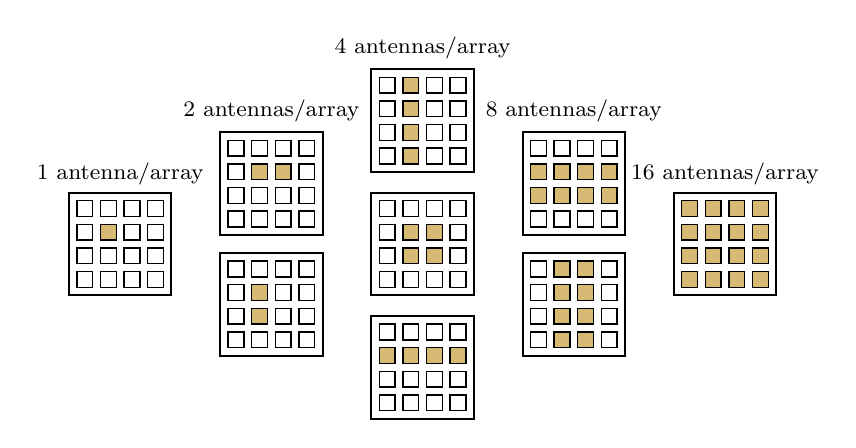
\begin{tikzpicture}[every node/.append style={font=\fontsize{11}{14}\selectfont}]


%%% DEFINITIONS %%%%%%%%%%%%%%%%%%%%%%%%%%%%%%%%%%%%%%%%%%%%%%%%%%%%%%%%%%%%%

% https://associatie.kuleuven.be/huisstijl/kleuren
\definecolor{blue1}{RGB}{0,64,122}
\definecolor{blue2}{RGB}{82,189,236}
\definecolor{red1}{RGB}{196, 30, 58}
\definecolor{red2}{RGB}{238, 75, 43}
\definecolor{red3}{RGB}{220, 20, 60}

\definecolor{gray1}{RGB}{180,180,180}
\definecolor{gray2}{RGB}{140,140,140}
\definecolor{cyan1}{RGB}{27, 221, 242}
\definecolor{orange1}{RGB}{221,138,46}
\definecolor{orange2}{RGB}{232,179,3}
\definecolor{brown1}{RGB}{84,40,17}
\definecolor{copper}{RGB}{184, 115, 51}
\definecolor{gold}{RGB}{214, 185, 114}
	

\def\RoomLength{9.15}
\def\RoomWidth{6.00}
\def\SideWbWidth{1.80}
\def\WindowWidth{1.35}

\def\TableWidth{1.40}
\def\TableDepth{.70}
\def\TableSpacing{.70}
\def\TableOffset{1.50}
\def\EisleWidth{.90}

\def\OrientationOffset{90} % Calibrate 0 orientation to north

\def\NodeSize{0.12}

\def\antennaSize{.2}
\def\arraySize{\antennaSize*6.5}
\def\arrayRegion{\antennaSize*8}
\newcommand\Square[1]{+(-#1,-#1) rectangle +(#1,#1)}

%%% DRAWING %%%%%%%%%%%%%%%%%%%%%%%%%%%%%%%%%%%%%%%%%%%%%%%%%%%%%%%%%%%%%%%%%

% 1x1
\def\xoffset{1.20*0*\arrayRegion}
\def\yoffset{0*\arrayRegion}
\def\y{2}
\foreach \x in {1,...,1}{
    \draw[fill=gold] (\xoffset+\x*\antennaSize*1.5,\yoffset+\y*\antennaSize*1.5) rectangle ++ (\antennaSize, \antennaSize);
}
\draw[draw=black, line width=0.75] (\xoffset-\antennaSize*0.5,\yoffset-\antennaSize*0.5) rectangle ++ (\antennaSize*6.5, \antennaSize*6.5);
\foreach \y in {0,...,3}{
    \foreach \x in {0,...,3}{
        \draw[draw=black, line width=0.50] (\xoffset+\x*\antennaSize*1.5,\yoffset+\y*\antennaSize*1.5) rectangle ++ (\antennaSize, \antennaSize);
    }
}

% 1x2
\def\xoffset{1.20*1*\arrayRegion}
\def\yoffset{0.48*\arrayRegion}
\def\y{2}
\foreach \x in {1,...,2}{
    \draw[fill=gold] (\xoffset+\x*\antennaSize*1.5,\yoffset+\y*\antennaSize*1.5) rectangle ++ (\antennaSize, \antennaSize);
}
\draw[draw=black, line width=0.75] (\xoffset-\antennaSize*0.5,\yoffset-\antennaSize*0.5) rectangle ++ (\antennaSize*6.5, \antennaSize*6.5);
\foreach \y in {0,...,3}{
    \foreach \x in {0,...,3}{
        \draw[draw=black, line width=0.50] (\xoffset+\x*\antennaSize*1.5,\yoffset+\y*\antennaSize*1.5) rectangle ++ (\antennaSize, \antennaSize);
    }
}


% 2x1
\def\xoffset{1.20*1*\arrayRegion}
\def\yoffset{-0.48*\arrayRegion}
\def\x{1}
\foreach \y in {1,...,2}{
    \draw[fill=gold] (\xoffset+\x*\antennaSize*1.5,\yoffset+\y*\antennaSize*1.5) rectangle ++ (\antennaSize, \antennaSize);
}
\draw[draw=black, line width=0.75] (\xoffset-\antennaSize*0.5,\yoffset-\antennaSize*0.5) rectangle ++ (\antennaSize*6.5, \antennaSize*6.5);
\foreach \y in {0,...,3}{
    \foreach \x in {0,...,3}{
        \draw[draw=black, line width=0.50] (\xoffset+\x*\antennaSize*1.5,\yoffset+\y*\antennaSize*1.5) rectangle ++ (\antennaSize, \antennaSize);
    }
}

% 1x4
\def\xoffset{1.20*2*\arrayRegion}
\def\yoffset{-0.98*\arrayRegion}
\def\y{2}
\foreach \x in {0,...,3}{
    \draw[fill=gold] (\xoffset+\x*\antennaSize*1.5,\yoffset+\y*\antennaSize*1.5) rectangle ++ (\antennaSize, \antennaSize);
}
\draw[draw=black, line width=0.75] (\xoffset-\antennaSize*0.5,\yoffset-\antennaSize*0.5) rectangle ++ (\antennaSize*6.5, \antennaSize*6.5);
\foreach \y in {0,...,3}{
    \foreach \x in {0,...,3}{
        \draw[draw=black, line width=0.50] (\xoffset+\x*\antennaSize*1.5,\yoffset+\y*\antennaSize*1.5) rectangle ++ (\antennaSize, \antennaSize);
    }
}

% 4x1
\def\xoffset{1.20*2*\arrayRegion}
\def\yoffset{0.98*\arrayRegion}
\def\x{1}
\foreach \y in {0,...,3}{
    \draw[fill=gold] (\xoffset+\x*\antennaSize*1.5,\yoffset+\y*\antennaSize*1.5) rectangle ++ (\antennaSize, \antennaSize);
}
\draw[draw=black, line width=0.75] (\xoffset-\antennaSize*0.5,\yoffset-\antennaSize*0.5) rectangle ++ (\antennaSize*6.5, \antennaSize*6.5);
\foreach \y in {0,...,3}{
    \foreach \x in {0,...,3}{
        \draw[draw=black, line width=0.50] (\xoffset+\x*\antennaSize*1.5,\yoffset+\y*\antennaSize*1.5) rectangle ++ (\antennaSize, \antennaSize);
    }
}

% 2x2
\def\xoffset{1.20*2*\arrayRegion}
\def\yoffset{0*\arrayRegion}
\foreach \y in {1,...,2}{
    \foreach \x in {1,...,2}{
        \draw[fill=gold] (\xoffset+\x*\antennaSize*1.5,\yoffset+\y*\antennaSize*1.5) rectangle ++ (\antennaSize, \antennaSize);
    }
}
\draw[draw=black, line width=0.75] (\xoffset-\antennaSize*0.5,\yoffset-\antennaSize*0.5) rectangle ++ (\antennaSize*6.5, \antennaSize*6.5);
\foreach \y in {0,...,3}{
    \foreach \x in {0,...,3}{
        \draw[draw=black, line width=0.50] (\xoffset+\x*\antennaSize*1.5,\yoffset+\y*\antennaSize*1.5) rectangle ++ (\antennaSize, \antennaSize);
    }
}

% 2x4
\def\xoffset{1.20*3*\arrayRegion}
\def\yoffset{0.48*\arrayRegion}
\foreach \y in {1,...,2}{
    \foreach \x in {0,...,3}{
        \draw[fill=gold] (\xoffset+\x*\antennaSize*1.5,\yoffset+\y*\antennaSize*1.5) rectangle ++ (\antennaSize, \antennaSize);
    }
}
\draw[draw=black, line width=0.75] (\xoffset-\antennaSize*0.5,\yoffset-\antennaSize*0.5) rectangle ++ (\antennaSize*6.5, \antennaSize*6.5);
\foreach \y in {0,...,3}{
    \foreach \x in {0,...,3}{
        \draw[draw=black, line width=0.50] (\xoffset+\x*\antennaSize*1.5,\yoffset+\y*\antennaSize*1.5) rectangle ++ (\antennaSize, \antennaSize);
    }
}

% 4x2
\def\xoffset{1.20*3*\arrayRegion}
\def\yoffset{-0.48*\arrayRegion}
\foreach \y in {0,...,3}{
    \foreach \x in {1,...,2}{
        \draw[fill=gold] (\xoffset+\x*\antennaSize*1.5,\yoffset+\y*\antennaSize*1.5) rectangle ++ (\antennaSize, \antennaSize);
    }
}
\draw[draw=black, line width=0.75] (\xoffset-\antennaSize*0.5,\yoffset-\antennaSize*0.5) rectangle ++ (\antennaSize*6.5, \antennaSize*6.5);
\foreach \y in {0,...,3}{
    \foreach \x in {0,...,3}{
        \draw[draw=black, line width=0.50] (\xoffset+\x*\antennaSize*1.5,\yoffset+\y*\antennaSize*1.5) rectangle ++ (\antennaSize, \antennaSize);
    }
}

% 4x4
\def\xoffset{1.20*4*\arrayRegion}
\def\yoffset{0*\arrayRegion}
\foreach \y in {0,...,3}{
    \foreach \x in {0,...,3}{
        \draw[fill=gold] (\xoffset+\x*\antennaSize*1.5,\y*\antennaSize*1.5) rectangle ++ (\antennaSize, \antennaSize);
    }
}
\draw[draw=black, line width=0.75] (\xoffset-\antennaSize*0.5,\yoffset-\antennaSize*0.5) rectangle ++ (\antennaSize*6.5, \antennaSize*6.5);
\foreach \y in {0,...,3}{
    \foreach \x in {0,...,3}{
        \draw[draw=black, line width=0.50] (\xoffset+\x*\antennaSize*1.5,\yoffset+\y*\antennaSize*1.5) rectangle ++ (\antennaSize, \antennaSize);
    }
}


\def\yoffset{-1.3*\arrayRegion}

\node[anchor=center, align=center, font=\footnotesize] at (1.20*0*\arrayRegion-\antennaSize*0.5+\arraySize*0.5, 0.9*\arrayRegion) {1 antenna/array};
\node[anchor=center, align=center, font=\footnotesize] at (1.20*1*\arrayRegion-\antennaSize*0.5+\arraySize*0.5, 1.4*\arrayRegion) {2 antennas/array};
\node[anchor=center, align=center, font=\footnotesize] at (1.20*2*\arrayRegion-\antennaSize*0.5+\arraySize*0.5, 1.9*\arrayRegion) {4 antennas/array};
\node[anchor=center, align=center, font=\footnotesize] at (1.20*3*\arrayRegion-\antennaSize*0.5+\arraySize*0.5, 1.4*\arrayRegion) {8 antennas/array};
\node[anchor=center, align=center, font=\footnotesize] at (1.20*4*\arrayRegion-\antennaSize*0.5+\arraySize*0.5, 0.9*\arrayRegion) {16 antennas/array};

\end{tikzpicture}

\end{document}